\documentclass[11pt,ignorenonframetext,]{beamer}
\setbeamertemplate{caption}[numbered]
\setbeamertemplate{caption label separator}{: }
\setbeamercolor{caption name}{fg=normal text.fg}
\beamertemplatenavigationsymbolsempty
\usepackage{lmodern}
\usepackage{amssymb,amsmath}
\usepackage{ifxetex,ifluatex}
\usepackage{fixltx2e} % provides \textsubscript
\ifnum 0\ifxetex 1\fi\ifluatex 1\fi=0 % if pdftex
  \usepackage[T1]{fontenc}
  \usepackage[utf8]{inputenc}
\else % if luatex or xelatex
  \ifxetex
    \usepackage{mathspec}
  \else
    \usepackage{fontspec}
  \fi
  \defaultfontfeatures{Ligatures=TeX,Scale=MatchLowercase}
\fi
\usetheme[]{metropolis}
% use upquote if available, for straight quotes in verbatim environments
\IfFileExists{upquote.sty}{\usepackage{upquote}}{}
% use microtype if available
\IfFileExists{microtype.sty}{%
\usepackage{microtype}
\UseMicrotypeSet[protrusion]{basicmath} % disable protrusion for tt fonts
}{}
\newif\ifbibliography
\hypersetup{
            pdftitle={Lecture 22},
            pdfauthor={Colin Rundel},
            pdfborder={0 0 0},
            breaklinks=true}
\urlstyle{same}  % don't use monospace font for urls
\usepackage{graphicx,grffile}
\makeatletter
\def\maxwidth{\ifdim\Gin@nat@width>\linewidth\linewidth\else\Gin@nat@width\fi}
\def\maxheight{\ifdim\Gin@nat@height>\textheight0.8\textheight\else\Gin@nat@height\fi}
\makeatother
% Scale images if necessary, so that they will not overflow the page
% margins by default, and it is still possible to overwrite the defaults
% using explicit options in \includegraphics[width, height, ...]{}
\setkeys{Gin}{width=\maxwidth,height=\maxheight,keepaspectratio}

% Prevent slide breaks in the middle of a paragraph:
\widowpenalties 1 10000
\raggedbottom

\AtBeginPart{
  \let\insertpartnumber\relax
  \let\partname\relax
  \frame{\partpage}
}
\AtBeginSection{
  \ifbibliography
  \else
    \let\insertsectionnumber\relax
    \let\sectionname\relax
    \frame{\sectionpage}
  \fi
}
\AtBeginSubsection{
  \let\insertsubsectionnumber\relax
  \let\subsectionname\relax
  \frame{\subsectionpage}
}

\setlength{\parindent}{0pt}
\setlength{\parskip}{6pt plus 2pt minus 1pt}
\setlength{\emergencystretch}{3em}  % prevent overfull lines
\providecommand{\tightlist}{%
  \setlength{\itemsep}{0pt}\setlength{\parskip}{0pt}}
\setcounter{secnumdepth}{0}

\usepackage{geometry}
\usepackage{graphicx}
\usepackage{amssymb}
\usepackage{color}          	% gives color options
\usepackage{url}		% produces hyperlinks
\usepackage[english]{babel}
\usepackage{colortbl}	% allows for color usage in tables
\usepackage{multirow}	% allows for rows that span multiple rows in tables
\usepackage{xcolor}		% this package has a variety of color options
\usepackage{calc}
\usepackage{multicol}
\usepackage{wrapfig}
\usepackage{textcomp}
\usepackage{bm}
\usepackage{bbm}
\usepackage{setspace}
\usepackage{changepage}
\usepackage{isotope}
\singlespacing

\usepackage{fontspec}
\newfontfamily\DejaSans{DejaVu Sans}

%%%%%%%%%%%%%%%%
% Small code output
%%%%%%%%%%%%%%%%

%% change fontsize of R code

\makeatletter
\@ifundefined{Shaded}{\newenvironment{Shaded}{}{}}{}
\makeatother


\let\oldShaded\Shaded
\let\endoldShaded\endShaded
\renewenvironment{Shaded}{\footnotesize\begin{spacing}{0.9}\oldShaded}{\endoldShaded\end{spacing}}

%% change fontsize of output
\let\oldverbatim\verbatim
\let\endoldverbatim\endverbatim
\renewenvironment{verbatim}{\footnotesize\begin{spacing}{0.9}\oldverbatim}{\endoldverbatim\end{spacing}}


\newcommand{\tinyoutput}{
  \renewenvironment{Shaded}{\tiny\begin{spacing}{0.9}\oldShaded}{\endoldShaded\end{spacing}}
  \renewenvironment{verbatim}{\tiny\begin{spacing}{0.9}\oldverbatim}{\endoldverbatim\end{spacing}}
}

\newcommand{\scriptoutput}{
  \renewenvironment{Shaded}{\scriptsize\begin{spacing}{0.9}\oldShaded}{\endoldShaded\end{spacing}}
  \renewenvironment{verbatim}{\scriptsize\begin{spacing}{0.9}\oldverbatim}{\endoldverbatim\end{spacing}}
}

\newcommand{\footnoteoutput}{
  \renewenvironment{Shaded}{\footnotesize\begin{spacing}{0.9}\oldShaded}{\endoldShaded\end{spacing}}
  \renewenvironment{verbatim}{\footnotesize\begin{spacing}{0.9}\oldverbatim}{\endoldverbatim\end{spacing}}
}

%\newcommand{\verbatimfont}[1]{\renewcommand{\verbatim@font}{\ttfamily#1}}


%%%%%%%%%%%%%%%%
% Custom Colors
%%%%%%%%%%%%%%%%

\definecolor{redhl}{rgb}{0.98,0.29,0.28}
\definecolor{yellowhl}{rgb}{0.98,0.87,0.28}
\newcommand{\hlr}[1]{\fcolorbox{redhl}{white}{$\displaystyle #1$}}
\newcommand{\hly}[1]{\fcolorbox{yellowhl}{white}{$\displaystyle #1$}}

\newcommand{\vvfill}{\vskip0pt plus 1filll}


\xdefinecolor{oiBlue}{rgb}{0.15, 0.35, 0.55}
\xdefinecolor{gray}{rgb}{0.5, 0.5, 0.5}
\xdefinecolor{darkGray}{rgb}{0.3, 0.3, 0.3}
\xdefinecolor{darkerGray}{rgb}{0.2, 0.2, 0.2}
\xdefinecolor{rubineRed}{rgb}{0.89,0,0.30}
\xdefinecolor{linkCol}{rgb}{0.11,0.49,0.95}	
\xdefinecolor{irishGreen}{rgb}{0,0.60,0}	
\xdefinecolor{darkturquoise}{rgb}{0.44, 0.58, 0.86}
\definecolor{lightGreen}{rgb}{0.533,0.765,0.42}
%\xdefinecolor{hlblue}{rgb}{0.051,0.65,1}
\xdefinecolor{hlblue}{rgb}{ 0.055, 0.639, 0.831}
\definecolor{light}{rgb}{.337,.608,.741}
\definecolor{dark}{rgb}{.337,.608,.741}

\definecolor{cpink}{rgb}{0.93, 0.23, 0.51}

%%%%%%%%%%%%%%%%
% Custom Commands
%%%%%%%%%%%%%%%%

% text colors
\newcommand{\red}[1]{\textit{\textcolor{rubineRed}{#1}}}
\newcommand{\orange}[1]{\textit{\textcolor{orange}{#1}}}
\newcommand{\pink}[1]{\textit{\textcolor{rubineRed!90!white!50}{#1}}}
\newcommand{\green}[1]{\textit{\textcolor{irishGreen}{#1}}}
\newcommand{\blue}[1]{\textit{\textcolor{darkturquoise}{#1}}}
\newcommand{\light}[1]{\textcolor{light}{\textbf{#1}}}
\newcommand{\dark}[1]{\textcolor{dark}{#1}}
\newcommand{\gray}[1]{\textcolor{gray}{#1}}


% links: webURL, webLin, appLink
\newcommand{\webURL}[1]{\urlstyle{same}{\textit{\textcolor{linkCol}{\url{#1}}} }}
\newcommand{\webLink}[2]{\href{#1}{\textcolor{linkCol}{{#2}}}}
\newcommand{\appLink}[2]{\href{#1}{\textcolor{lightGreen!80!black!90}{{#2}}}}

% mail
\newcommand{\mail}[1]{\href{mailto:#1}{\textit{\textcolor{linkCol}{#1}}}}

% highlighting: hl, hlGr, mathhl
\newcommand{\hl}[1]{\textit{\textcolor{hlblue}{#1}}}
\newcommand{\hlGr}[1]{\textit{\textcolor{lightGreen}{#1}}}
\newcommand{\hlRd}[1]{\textit{\textcolor{rubineRed}{#1}}}
\newcommand{\mathhl}[1]{\textcolor{hlblue}{\ensuremath{#1}}}

% example
\newcommand{\ex}[1]{\textcolor{blue}{{{\small (#1)}}}}


\DeclareMathOperator*{\argmin}{arg\,min}
\DeclareMathOperator*{\argmax}{arg\,max}

\title{Lecture 22}
\subtitle{Computational Methods for GPs}
\author{Colin Rundel}
\date{04/12/2017}

\begin{document}
\frame{\titlepage}

\section{GPs and Computational
Complexity}\label{gps-and-computational-complexity}

\begin{frame}{The problem with GPs}

Unless you are lucky (or clever), Gaussian process models are difficult
to scale to large problems. For a Gaussian process
\(\bm{y} \sim \mathcal{N}(\bm{\mu},\bm{\Sigma})\):

\pause

\vspace{3mm}

Want to sample \(\bm{y}\)?
\[ \bm{\mu} + \hlr{\text{Chol}(\bm{\Sigma})} \times \bm{Z} \text{ with } Z_i \sim \mathcal{N}(0,1) \qquad \qquad \color{redhl}{\mathcal{O}\left(n^3\right)} \]

\pause

Evaluate the (log) likelihood?
\[ -\frac{1}{2} \log \hlr{|\Sigma|} - \frac{1}{2} (\bm{x}-\bm{\mu})' \hlr{\bm{\Sigma}^{-1}} (\bm{x}-\bm{\mu}) - \frac{n}{2}\log 2\pi \qquad \qquad \color{redhl}{\mathcal{O}\left(n^3\right)}\]

\pause

Update covariance parameter?
\[ \hly{\{\Sigma\}_{ij}} = \sigma^2 \exp(-\{d\}_{ij}\phi) + \sigma^2_n \, 1_{i=j} \qquad \qquad \color{yellowhl}{\mathcal{O}\left(n^2\right)}\]

\end{frame}

\begin{frame}{A simple guide to computational complexity}

\Large

\begin{center}
\vfill
$\mathcal{O}\left(n\right)$ - Linear complexity \pause- Go for it \pause

\vspace{15mm}

$\mathcal{O}\left(n^2\right)$ - Quadratic complexity \pause- Pray \pause

\vspace{15mm}

$\mathcal{O}\left(n^3\right)$ - Cubic complexity \pause- Give up

\vfill
\end{center}

\end{frame}

\begin{frame}{How bad is the problem?}

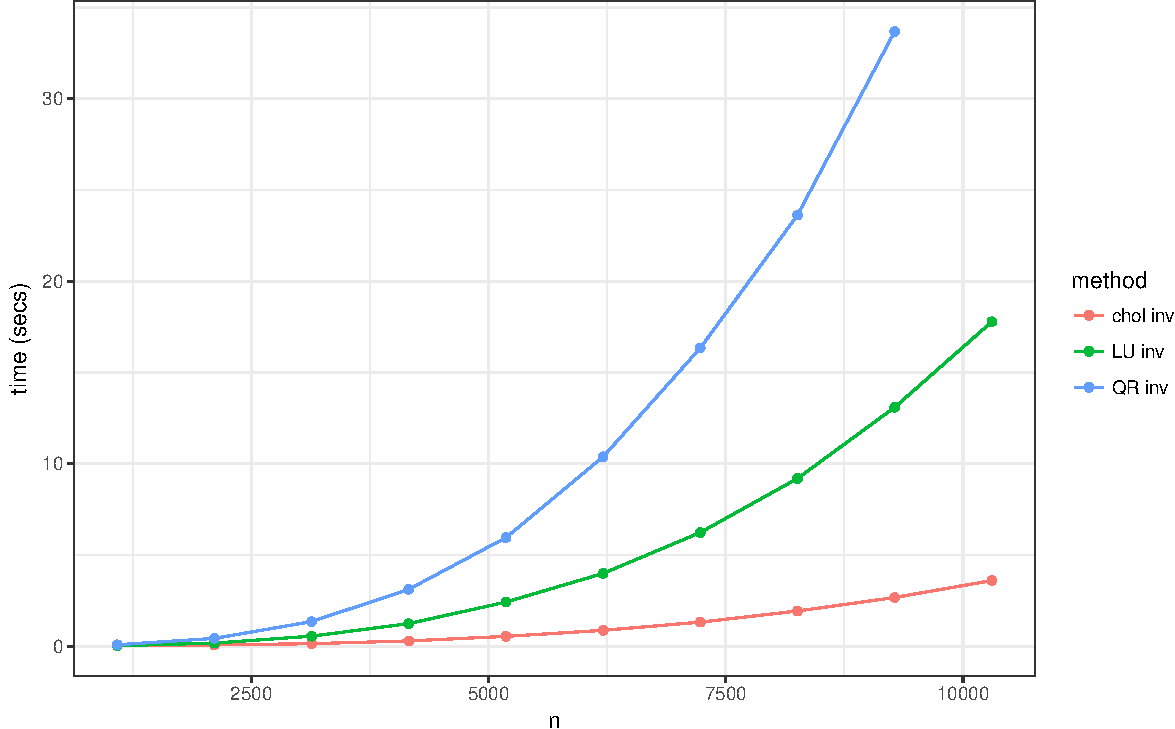
\includegraphics{Lec22_files/figure-beamer/unnamed-chunk-1-1.pdf}

\end{frame}

\begin{frame}{Practice - Migratory Model Prediction}

After fitting the GP need to sample from the posterior predictive
distribution at \(\sim3000\) locations
\[ \bm{y}_{p} \sim \mathcal{N}\left(\mu_p + \Sigma_{po} \Sigma_o^{-1}(y_o - \mu_o) ,~ \Sigma_p - \Sigma_{po} \Sigma_{o}^{-1} \Sigma_{op}\right) \]

\pause

\scriptsize  

\begin{center}
\renewcommand*{\arraystretch}{1.5}
\begin{tabular}{rl|c|c|c}
& Step                                    & CPU (secs)  & CPU+GPU (secs)  & Rel. Performance \\
\hline
1. & Calc. $\Sigma_p$, $\Sigma_{po}$      & 1.080       & 0.046           & 23.0 \\
2. & Calc. $\text{chol}(\Sigma_p - \Sigma_{po} \Sigma_{o}^{-1} \Sigma_{op})$         
                                          & 0.467       & 0.208           & 2.3 \\
3. & Calc. $\mu_{p|o} + \text{chol}(\Sigma_{p|o}) \times Z$
                                          & 0.049       & 0.052           & 0.9 \\
4. & Calc. Allele Prob                    & 0.129       & 0.127           & 1.0 \\
\hline 
   & Total                                & 1.732       & 0.465           & 3.7 \\
\end{tabular}
\end{center}

\vspace{3mm}

\normalsize
Total run time: CPU (28.9 min), CPU+GPU (7.8 min)

\end{frame}

\begin{frame}{Cholesky CPU vs GPU (P100)}

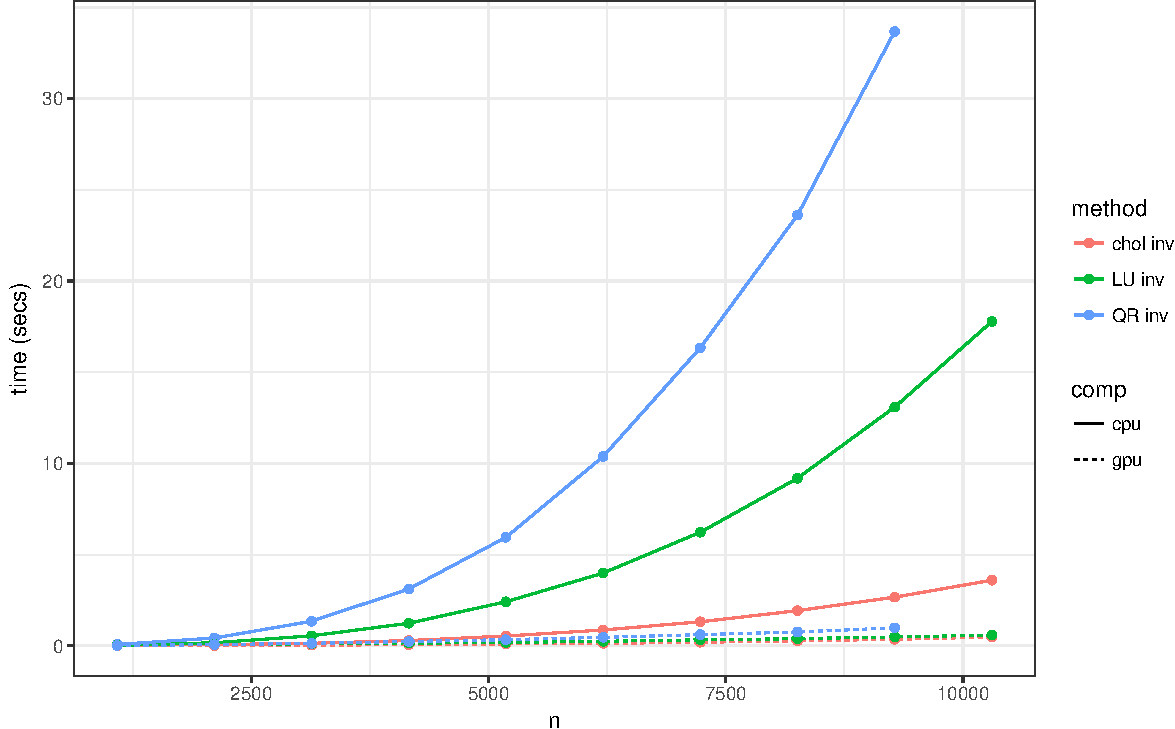
\includegraphics{Lec22_files/figure-beamer/unnamed-chunk-2-1.pdf}

\end{frame}

\begin{frame}{}

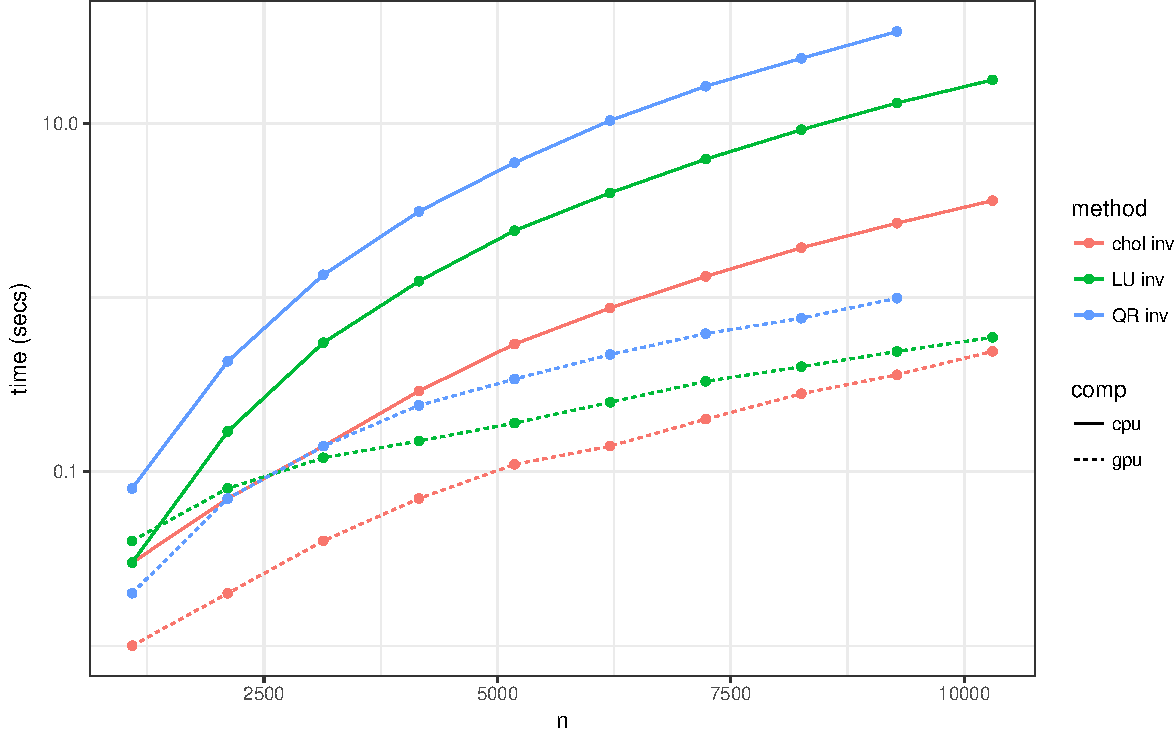
\includegraphics{Lec22_files/figure-beamer/unnamed-chunk-3-1.pdf}

\end{frame}

\begin{frame}{Relative Performance}

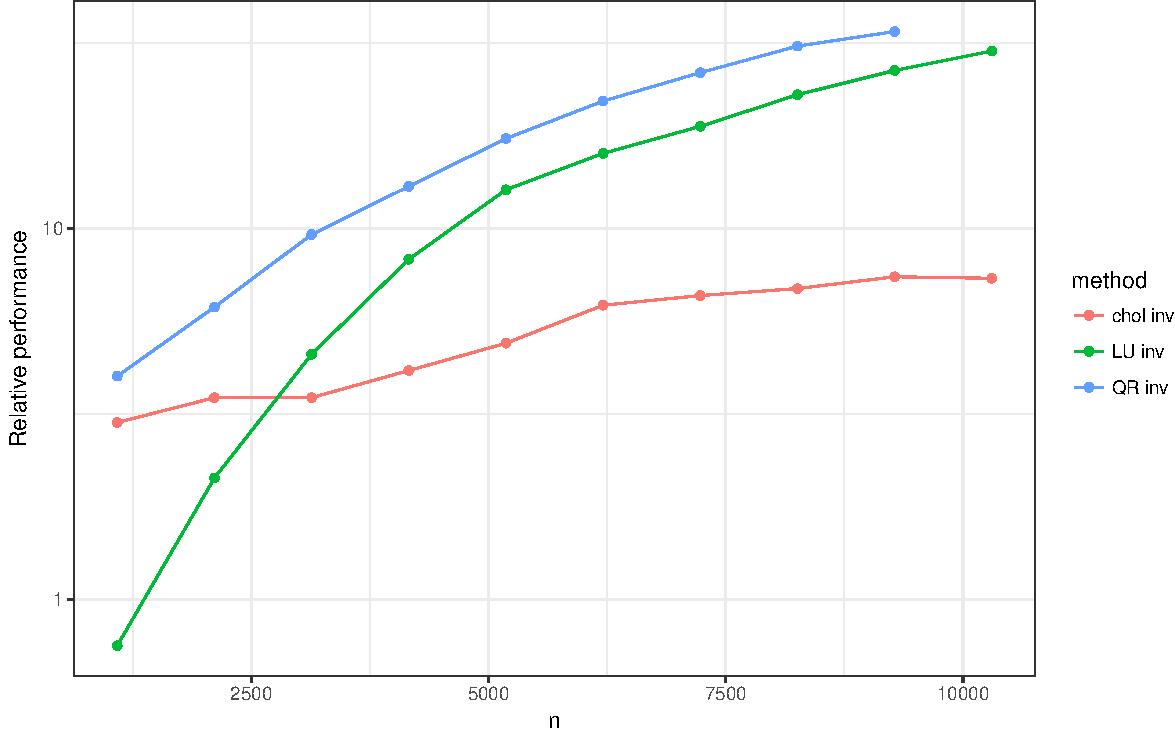
\includegraphics{Lec22_files/figure-beamer/unnamed-chunk-4-1.pdf}

\end{frame}

\begin{frame}{Aside - Matrix Multiplication}

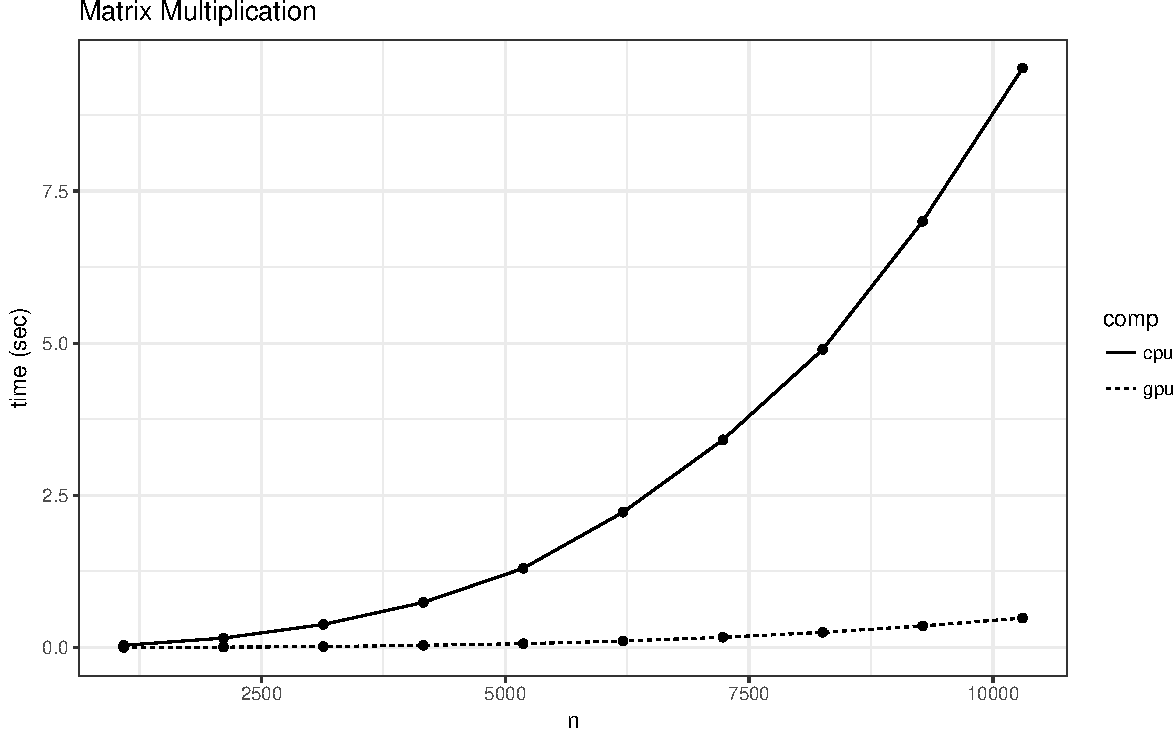
\includegraphics{Lec22_files/figure-beamer/unnamed-chunk-5-1.pdf}

\end{frame}

\begin{frame}[fragile]{An even bigger hammer}

\small
\texttt{bigGP} is an R package written by Chris Paciorek (UC Berkeley),
et al.

\begin{itemize}
\item
  Specialized distributed implementation of linear algebra operation for
  GPs
\item
  Designed to run on large super computer clusters
\item
  Uses both shared and distributed memory
\item
  Able to fit models on the order of \(n = 65\)k (32 GB Cov. matrix)
\end{itemize}

\vspace{-3mm}

\begin{center}
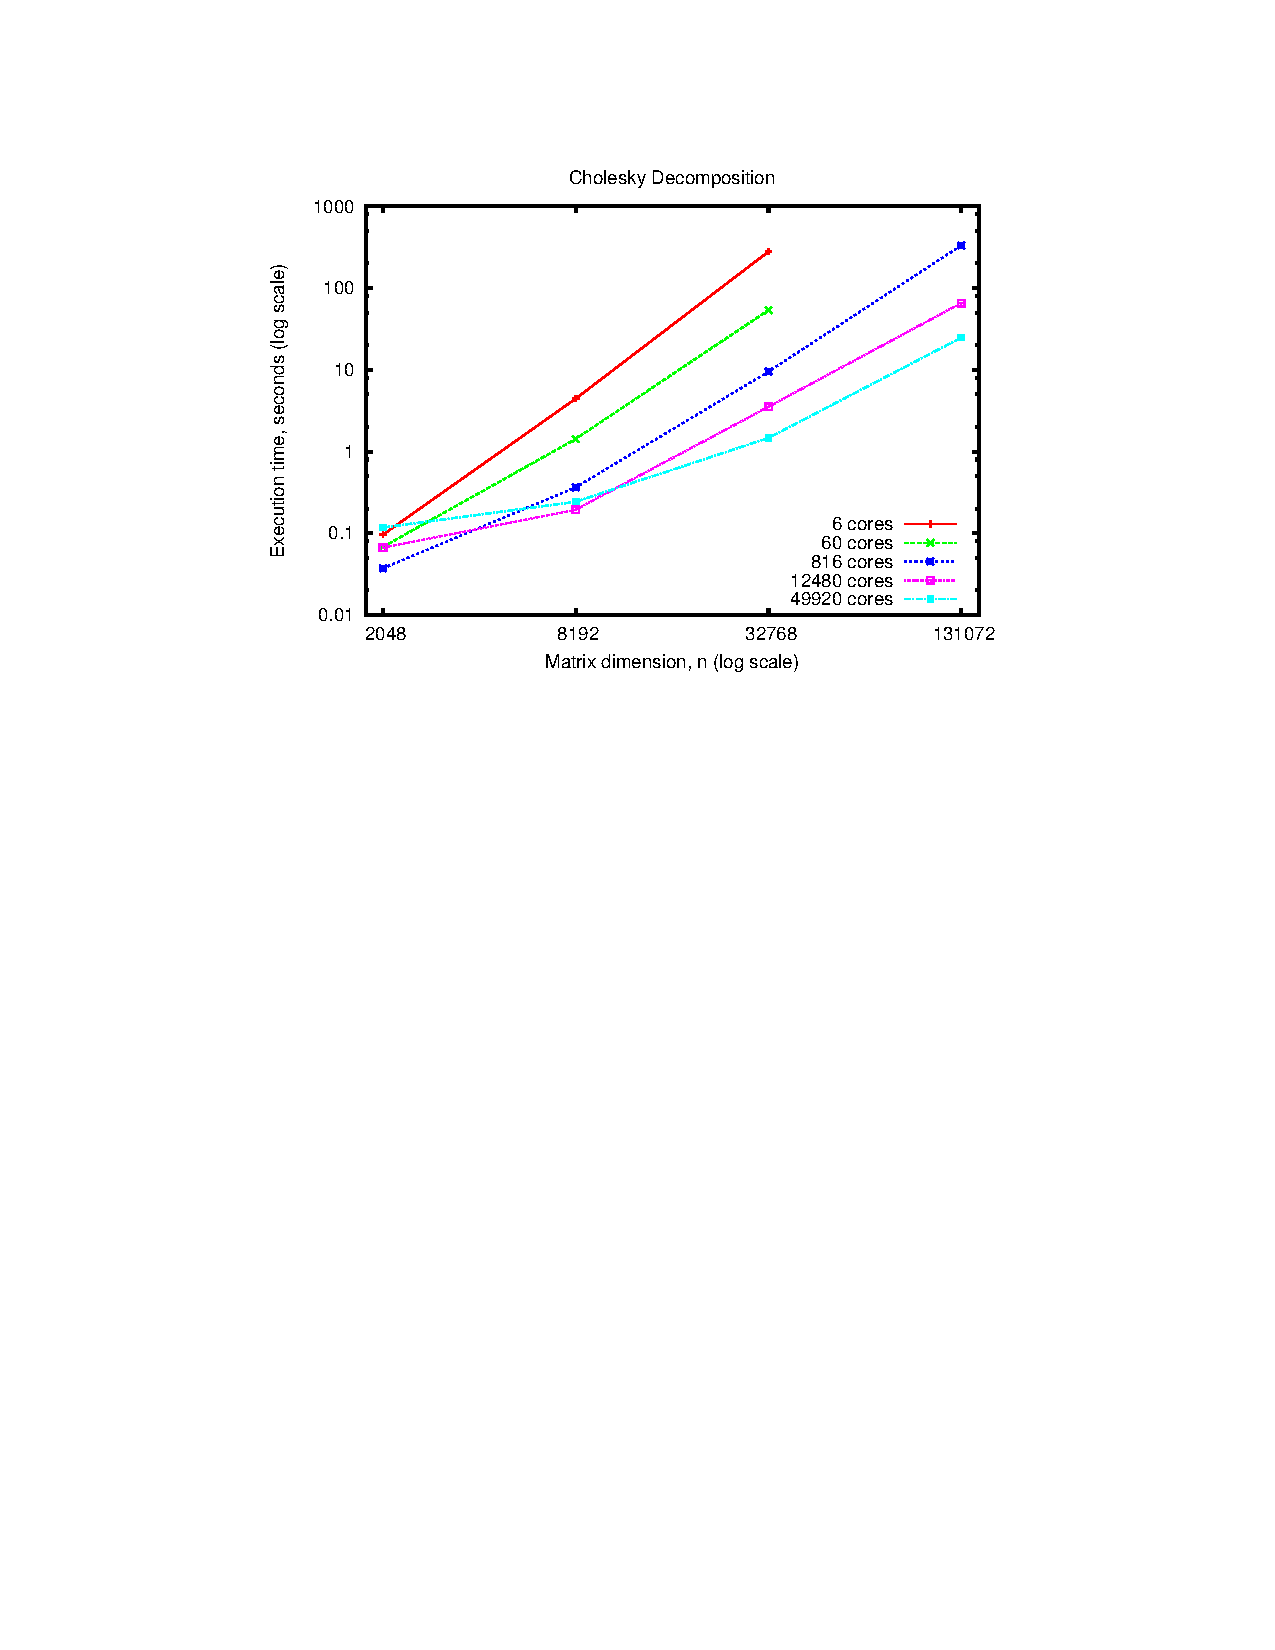
\includegraphics[width=0.7\textwidth]{figs/Paciorek.pdf}
\end{center}

\end{frame}

\begin{frame}{More scalable solutions?}

\large

\begin{itemize}
\tightlist
\item
  Spectral domain / basis functions
\end{itemize}

\vspace{3mm}

\begin{itemize}
\tightlist
\item
  Covariance tapering
\end{itemize}

\vspace{3mm}

\begin{itemize}
\tightlist
\item
  GMRF approximations
\end{itemize}

\vspace{3mm}

\begin{itemize}
\tightlist
\item
  Low-rank approximations
\end{itemize}

\vspace{3mm}

\begin{itemize}
\tightlist
\item
  Nearest-neighbor models
\end{itemize}

\end{frame}

\section{Low Rank Approximations}\label{low-rank-approximations}

\begin{frame}{Low rank approximations in general}

Lets look at the example of the singular value decomposition of a
matrix,

\[ \underset{n \times m}{M} = \underset{n \times n}{U}\,\underset{n \times m}{\text{diag}(S)}\,\underset{m \times m}{V^{\,t}} \]
where \(U\) are called the left singular vectors, \(V\) the right
singular vectors, and \(S\) the singular values. Usually the singular
values and vectors are ordered such that the signular values are in
descending order.

\pause

It turns out (Eckart--Young theorem) that we can approximate \(M\) as
having rank \(r\) by defining \(\tilde S\) to only have the \(r\)
largest singular values (others set to zero).

\[ 
\begin{aligned}
\underset{n \times m}{\tilde M} 
  &= \underset{n \times n}{U}\,\underset{n \times m}{\text{diag}(\tilde S)}\,\underset{m \times m}{V^{\,t}} 
  &= \underset{n \times k}{\tilde U}\,\underset{k \times k}{\text{diag}(\tilde S)}\,\underset{k \times m}{\tilde{V}^{\,t}} 
\end{aligned}
\]

\end{frame}

\begin{frame}{Example}

\footnotesize

\[ \begin{aligned}
M 
&= \begin{pmatrix}
  1.000 & 0.500 & 0.333 & 0.250 \\ 
  0.500 & 0.333 & 0.250 & 0.200 \\ 
  0.333 & 0.250 & 0.200 & 0.167 \\ 
  0.250 & 0.200 & 0.167 & 0.143 \\ 
\end{pmatrix} 
  = U \, \text{diag}(S) \, V^{\,t} \\
U = V &= \begin{pmatrix}
  -0.79 & 0.58 & -0.18 & -0.03 \\ 
  -0.45 & -0.37 & 0.74 & 0.33 \\ 
  -0.32 & -0.51 & -0.10 & -0.79 \\ 
  -0.25 & -0.51 & -0.64 & 0.51 \\ 
  \end{pmatrix} \\
S &= 
\begin{pmatrix} 1.50 & 0.17  & 0.01 & 0.00 \end{pmatrix}
\end{aligned} \]

\pause

\normalsize
Rank 2 approximation: \footnotesize
\[ \begin{aligned}
\tilde M
&= \begin{pmatrix}
  -0.79 &  0.58 \\ 
  -0.45 & -0.37 \\ 
  -0.32 & -0.51 \\ 
  -0.25 & -0.51 \\ 
\end{pmatrix}
\begin{pmatrix}
  1.50 & 0.00 \\ 
  0.00 & 0.17 \\ 
\end{pmatrix}
\begin{pmatrix}
  -0.79 & -0.45 & -0.32 & -0.25 \\ 
  0.58 & -0.37 & -0.51 & -0.51 \\ 
\end{pmatrix} \\
&= 
\begin{pmatrix}
  1.000 & 0.501 & 0.333 & 0.249 \\ 
  0.501 & 0.330 & 0.251 & 0.203 \\ 
  0.333 & 0.251 & 0.200 & 0.166 \\ 
  0.249 & 0.203 & 0.166 & 0.140 \\ 
\end{pmatrix}
\end{aligned} \]

\end{frame}

\begin{frame}{Approximation Error}

We can measure the error of the approximation using the Frobenius norm,
\[ \lVert M-\tilde M\rVert_F = \left( \sum_{i=1}^m\sum_{j=1}^n (M_{ij}-\tilde M_{ij})^2\right)^{1/2} \]

\pause

\vspace{3mm}

Strong dependence (large eff. range):

\vspace{2mm}

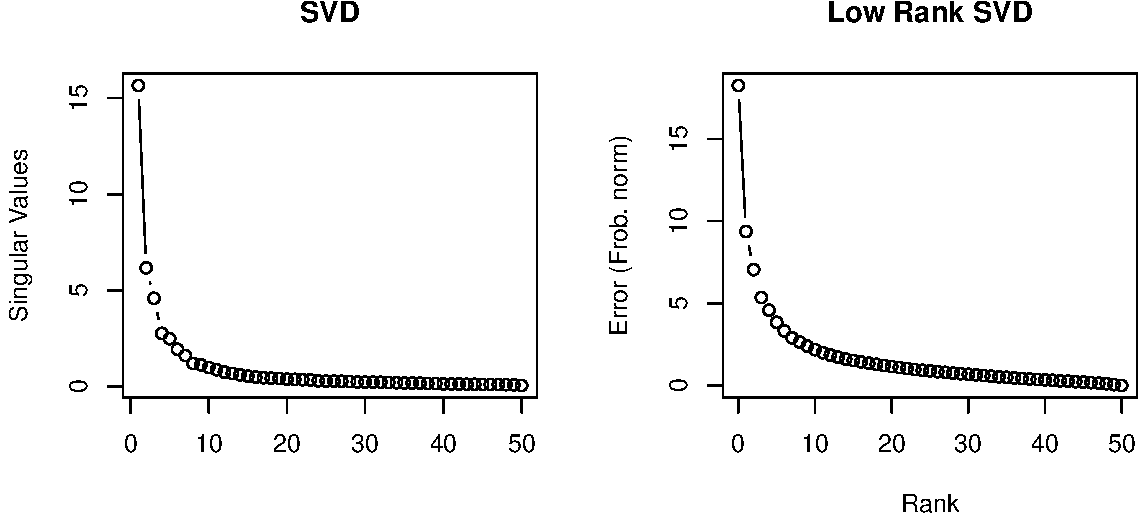
\includegraphics{Lec22_files/figure-beamer/unnamed-chunk-7-1.pdf}

\end{frame}

\begin{frame}{}

Weak dependence (short eff. range):

\vspace{2mm}

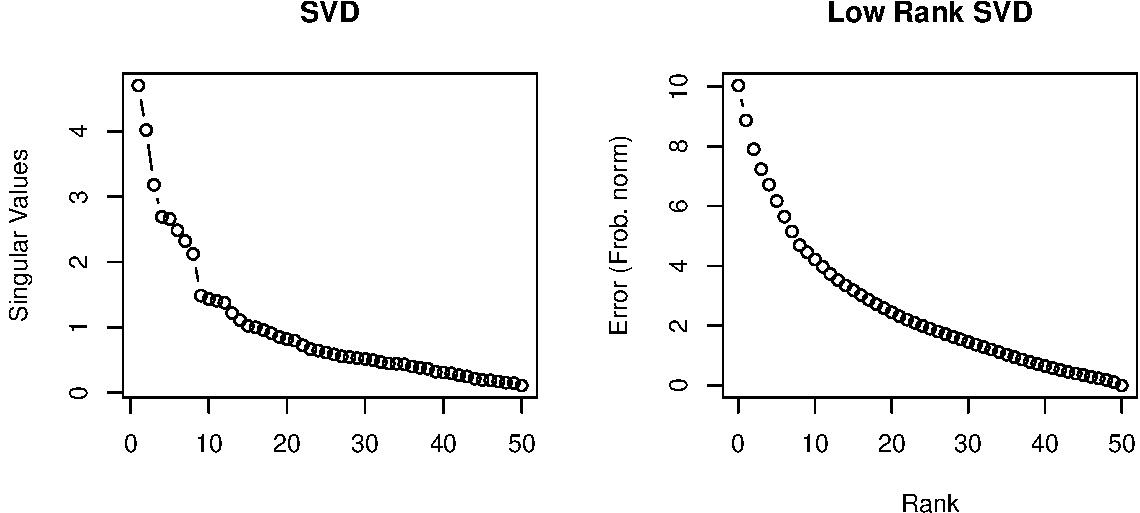
\includegraphics{Lec22_files/figure-beamer/unnamed-chunk-8-1.pdf}

\end{frame}

\begin{frame}[t]{How does this help? (Sherman-Morrison-Woodbury)}

There is an immensely useful linear algebra identity, the
Sherman-Morrison-\emph{Woodbury} formula, for the inverse (and
determinant) of a decomposed matrix,

\[\begin{aligned}
\underset{n \times m}{\tilde M}^{-1} 
&= \left(\underset{n \times m}{A} + \underset{n \times k}{U} ~ \underset{k \times k}{S} ~ \underset{k \times m}{V^t}\right)^{-1} \\
&= A^{-1} - A^{-1} U \left(S^{-1}+V^{\,t} A^{-1} U\right)^{-1}V^{\,t} A^{-1}.
\end{aligned}\]

\pause

How does this help?

\begin{itemize}
\item
  Imagine that \(A = \text{diag}(A)\), then it is trivial to find
  \(A^{-1}\).
\item
  \(S^{-1}\) is \(k \times k\) which is hopefully small, or even better
  \(S = \text{diag}(S)\).
\item
  \(\left(S^{-1}+V^{\,t} A^{-1} U\right)\) is \(k \times k\) which is
  hopefully small.
\end{itemize}

\end{frame}

\begin{frame}{Aside - Determinant}

Remember for any MVN distribution when evaluating the likelihood
\[ -\frac{1}{2} \log {|\Sigma|} - \frac{1}{2} (\bm{x}-\bm{\mu})' {\bm{\Sigma}^{-1}} (\bm{x}-\bm{\mu}) - \frac{n}{2}\log 2\pi\]
we need the inverse of \(\Sigma\) as well as its \emph{determinant}.

\pause

\begin{itemize}
\tightlist
\item
  For a full rank Cholesky decomposition we get the determinant for
  ``free''.
\end{itemize}

\vspace{-3mm}

\[|M| = |LL^t| = \prod_{i=1}^n \left(\text{diag}(L)_i\right)^2\]

\pause

\begin{itemize}
\tightlist
\item
  For a low rank approximation the Sherman-Morrison-Woodbury /
  Determinant lemma gives us,
\end{itemize}

\vspace{-3mm}

\[\begin{aligned}
\det(\tilde M) 
  &= \det({A} + {U} {S} {V^t}) \\
  &= \det(S^{-1} + V^t A^{-1} U) ~ \det(S) ~ \det(A)
\end{aligned}\]

\end{frame}

\begin{frame}[t]{Low rank approximations for GPs}

For a standard spatial random effects model,

\[ y(\bm{s}) = x(\bm{s}) \, \bm{\beta} + w(\bm{s}) + \epsilon, \quad \epsilon \sim N(0,~\tau^2 I) \]
\[ w(\bm{s}) \sim \mathcal{N}(0,~\bm{\Sigma}(\bm{s})), \quad \bm{\Sigma}(\bm{s},\bm{s}')=\sigma\,\rho(\bm{s},\bm{s}'|\theta) \]

if we can replace \(\bm{\Sigma}(\bm{s})\) with a low rank approximation
of the form

\begin{itemize}
\item
  \(\bm{\Sigma}(\bm{s}) \approx \bm{U}\,\bm{S}\,\bm{V}^t\) where
\item
  \(\bm{U}\) and \(\bm{V}\) are \(n \times k\),
\item
  \(\bm{S}\) is \(k \times k\), and
\item
  \(A = \tau^2 I\) or a similar diagonal matrix
\end{itemize}

\end{frame}

\section{Predictive Processes}\label{predictive-processes}

\begin{frame}{Gaussian Predictive Processes}

\small

For a rank \(k\) approximation,

\begin{itemize}
\item
  Pick \(k\) knot locations \(\bm{s}^\star\)
\item
  Calculate knot covariance, \(\bm{\Sigma}(\bm{s}^\star)\), and knot
  cross-covariance, \(\bm{\Sigma}(\bm{s}, \bm{s}^\star)\)
\item
  Approximate full covariance using
\end{itemize}

\vspace{-2mm}
\[ \bm{\Sigma}(\bm{s}) \approx \underset{n \times k}{\bm{\Sigma}(\bm{s},\bm{s}^\star)} \, \underset{k \times k}{\bm{\Sigma}(\bm{s}^\star)^{-1}} \, \underset{k \times n}{\bm{\Sigma}(\bm{s}^\star,\bm{s})}. \]

\begin{itemize}
\tightlist
\item
  PPs systematically underestimates variance (\(\sigma^2\)) and inflate
  \(\tau^2\), Modified predictive processs corrects this using
\end{itemize}

\vspace{-2mm} \[
\begin{aligned}
\bm{\Sigma}(\bm{s}) \approx &
\bm{\Sigma}(\bm{s},\bm{s}^\star) \, \bm{\Sigma}(\bm{s}^\star)^{-1} \, \bm{\Sigma}(\bm{s}^\star,\bm{s}) \\
&+ \text{diag}\Big(\bm{\Sigma}(\bm{s}) - \bm{\Sigma}(\bm{s},\bm{s}^\star) \, \bm{\Sigma}(\bm{s}^\star)^{-1} \, \bm{\Sigma}(\bm{s}^\star,\bm{s})\Big).
\end{aligned}
\]

\vspace{4mm}

\footnotesize

\begin{center}
Banerjee, Gelfand, Finley, Sang (2008) \quad Finley, Sang, Banerjee, Gelfand (2008)
\end{center}

\end{frame}

\begin{frame}{Example}

Below we have a surface generate from a squared exponential Gaussian
Process where

\[ \{\Sigma\}_{ij} = \sigma^2 \exp\left(-(\phi\,d)^2\right) + \tau^2 I \]
\[ \sigma^2 = 1 \quad \phi=9 \quad \tau^2 = 0.1 \]

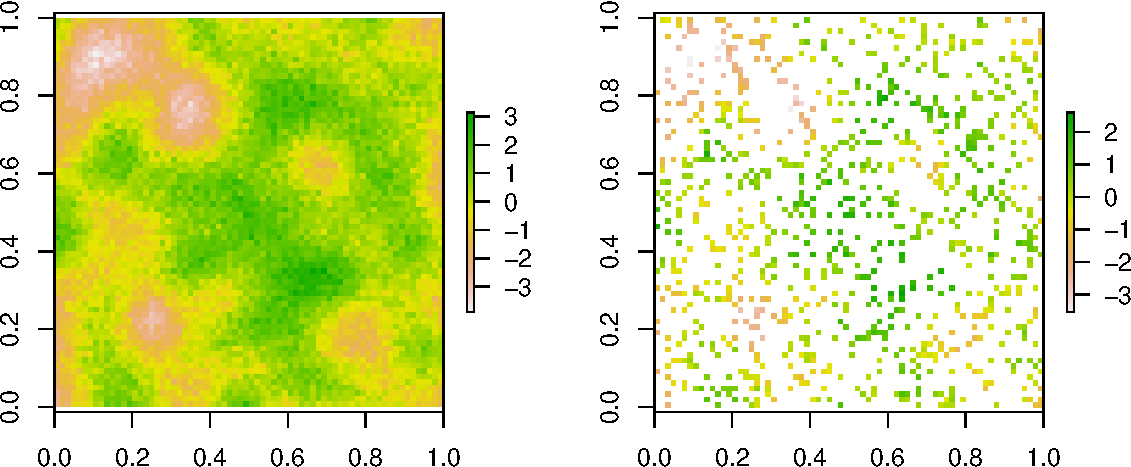
\includegraphics{Lec22_files/figure-beamer/unnamed-chunk-10-1.pdf}

\end{frame}

\begin{frame}{Predictive Process Model Results}

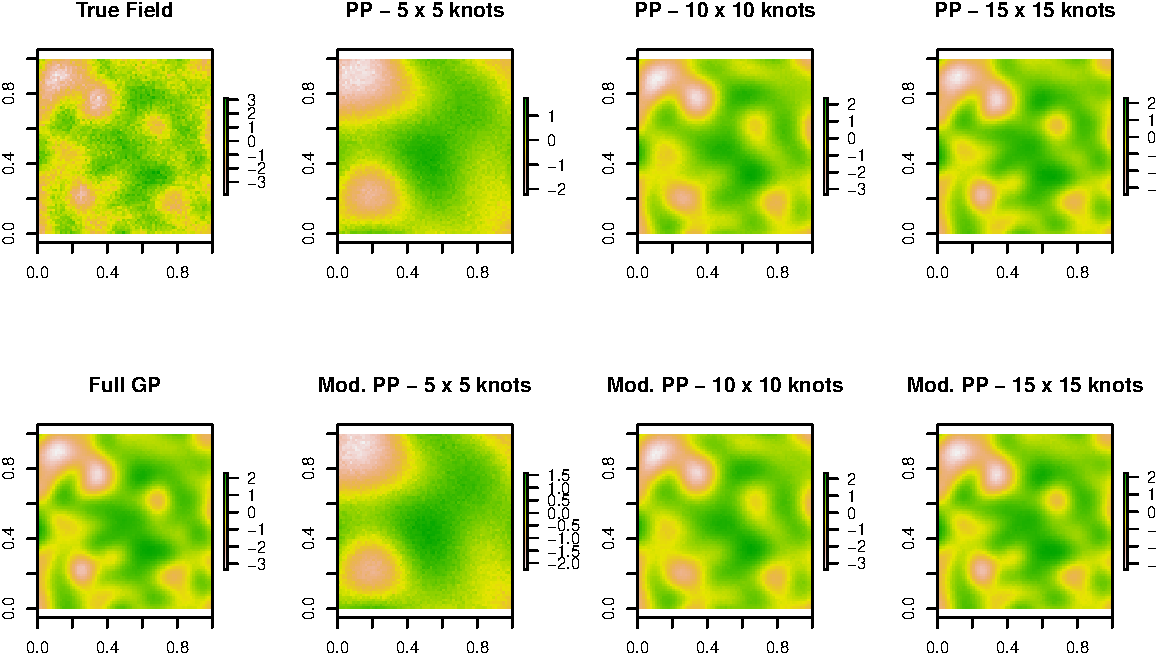
\includegraphics{Lec22_files/figure-beamer/unnamed-chunk-13-1.pdf}

\end{frame}

\begin{frame}{Performance}

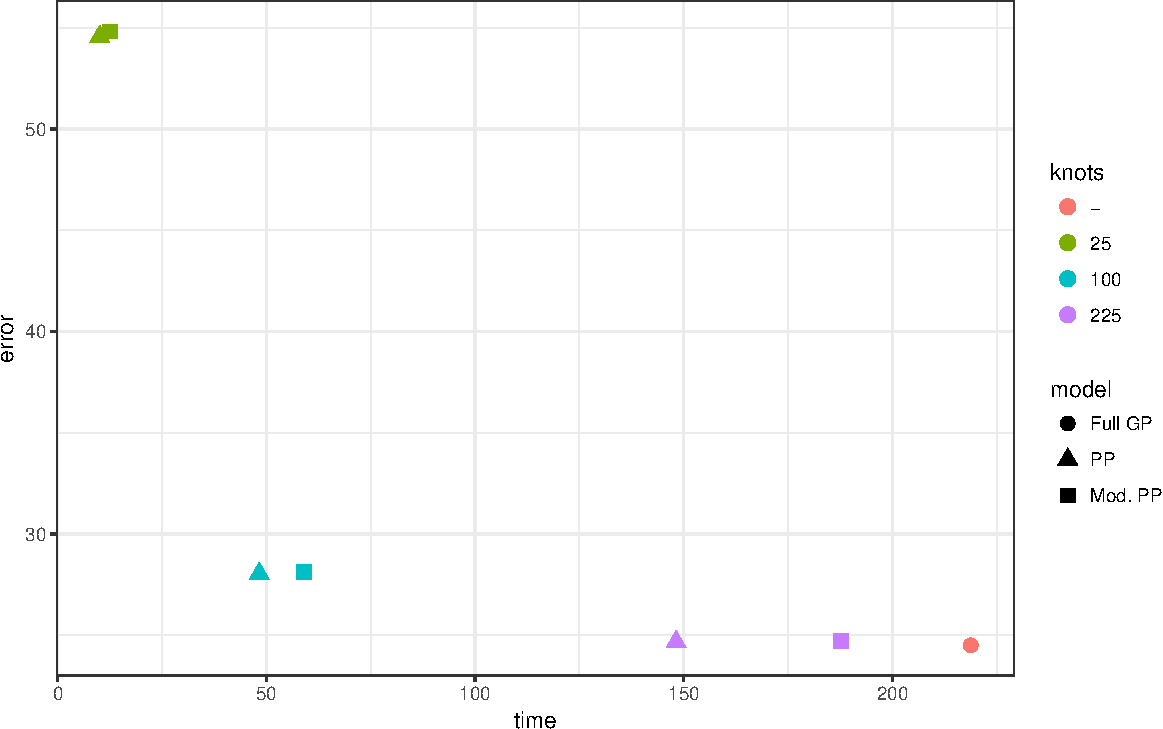
\includegraphics{Lec22_files/figure-beamer/unnamed-chunk-14-1.pdf}

\end{frame}

\begin{frame}{Parameter Estimates}

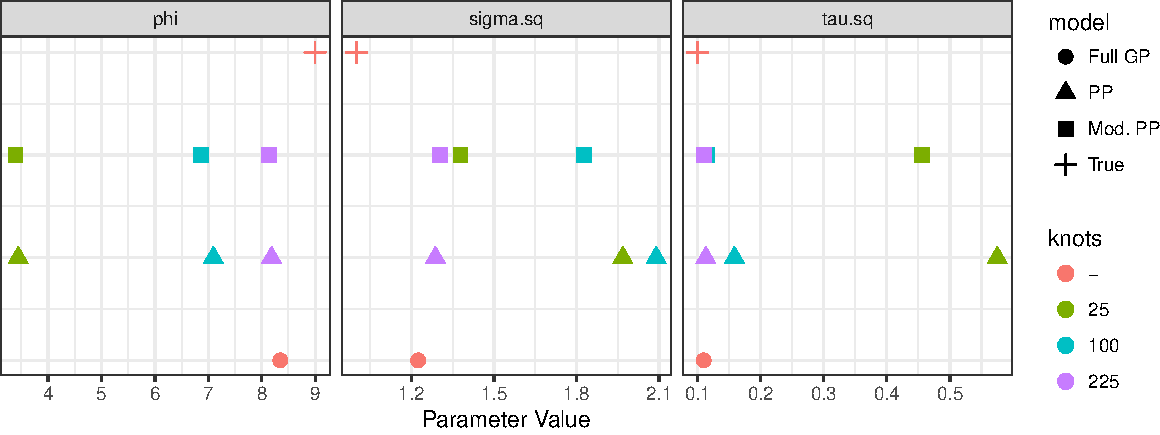
\includegraphics{Lec22_files/figure-beamer/unnamed-chunk-15-1.pdf}

\end{frame}

\section{Random Projections}\label{random-projections}

\begin{frame}{Low Rank Approximations via Random Projections}

\begin{enumerate}
\def\labelenumi{\arabic{enumi}.}
\item
  Starting with an \(m \times n\) matrix \(\bm{A}\).
\item
  Draw an \(n \times k+p\) Gaussian random matrix \(\bm{\Omega}\).
\item
  Form \(\bm{Y} = \bm{A}\,\bm{\Omega}\) and compute its QR factorization
  \(\bm{Y} = \bm{Q}\,\bm{R}\)
\end{enumerate}

\begin{enumerate}
\def\labelenumi{\arabic{enumi}.}
\setcounter{enumi}{3}
\item
  Form the \(k+p \times n\) matrix \(\bm{B}=\bm{Q}'\,\bm{A}\).
\item
  Compute the SVD of the small matrix \(\bm{B}\),
  \(\bm{B} = \bm{\hat{U}}\,\bm{S}\,\bm{V}'\).
\item
  Form the matrix \(\bm{U} = \bm{Q} \, \bm{\hat{U}}\).
\end{enumerate}

\vspace{2mm}

Resulting approximation has a bounded expected error,

\[ \text{E } \, \| \bm{A} - \bm{U}\bm{S}\bm{V}'\| \leq \left[1 + \frac{4\sqrt{k+p}}{p-1} \sqrt{\min(m,n)} \right] \sigma_{k+1}. \]

\vvfill

\footnotesize

\begin{center}
Halko, Martinsson, Tropp (2011)
\end{center}

\end{frame}

\begin{frame}{Random Matrix Low Rank Approximations and GPs}

Preceeding algorithm can be modified slightly to take advantage of the
positive definite structure of a covariance matrix.

\begin{enumerate}
\def\labelenumi{\arabic{enumi}.}
\item
  Starting with an \(n \times n\) covariance matrix \(\bm{A}\).
\item
  Draw an \(n \times k+p\) Gaussian random matrix \(\bm{\Omega}\).
\item
  Form \(\bm{Y} = \bm{A}\,\bm{\Omega}\) and compute its QR factorization
  \(\bm{Y} = \bm{Q}\,\bm{R}\)
\item
  Form the \(k+p \times k+p\) matrix
  \(\bm{B}=\bm{Q}'\,\bm{A} \, \bm{Q}\).
\item
  Compute the eigen decomposition of the small matrix \(\bm{B}\),
  \(\bm{B} = \bm{\hat{U}}\,\bm{S}\,\bm{\hat{U}}'\).
\item
  Form the matrix \(\bm{U} = \bm{Q} \, \bm{\hat{U}}\).
\end{enumerate}

Once again we have a bound on the error,

\[
   \text{E } \| \bm{A} - \bm{Q}(\bm{Q}'\bm{A}\bm{Q})\bm{Q}'\| 
 = \text{E } \| \bm{A} - \bm{U}\bm{S}\bm{U}'\| 
\lessapprox c \cdot \sigma_{k+1}. 
\]

\vvfill

\footnotesize

\begin{center}
Halko, Martinsson, Tropp (2011), Banerjee, Dunson, Tokdar (2012)
\end{center}

\end{frame}

\begin{frame}{Low Rank Approximations and GPUs}

Both predictive process and random matrix low rank approximations are
good candidates for acceleration using GPUs.

\vspace{3mm}

\begin{itemize}
\tightlist
\item
  Both use Sherman-Woodbury-Morrison to calculate the inverse (involves
  matrix multiplication, addition, and a small matrix inverse).
\end{itemize}

\vspace{3mm}

\begin{itemize}
\tightlist
\item
  Predictive processes involves several covariance matrix calculations
  (knots and cross-covariance) and a small matrix inverse.
\end{itemize}

\vspace{3mm}

\begin{itemize}
\tightlist
\item
  Random matrix low rank approximations involves a large matrix
  multiplication (\(\bm{A}\,\bm{\Omega}\)) and several small matrix
  decompositions (QR, eigen).
\end{itemize}

\end{frame}

\begin{frame}{Comparison (\(n=15,000\), \(k=\{100,\ldots,4900\}\))}

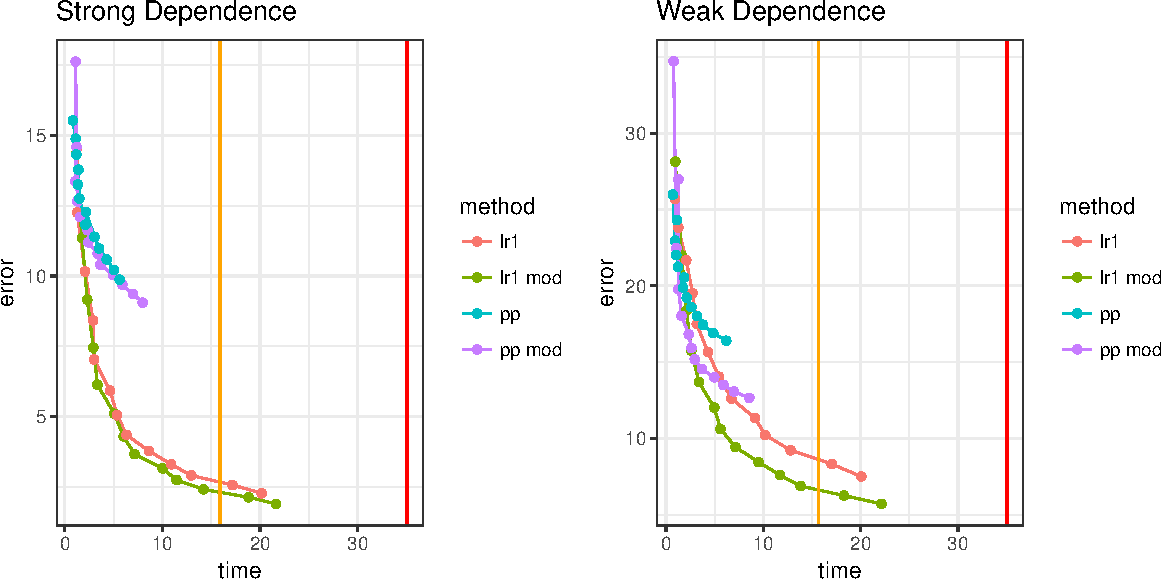
\includegraphics{Lec22_files/figure-beamer/unnamed-chunk-16-1.pdf}

\end{frame}

\begin{frame}[t]{Rand. Projection LR Decompositions for Prediction}

\small

This approach can also be used for prediction, if we want to sample

\[\bm{y} \sim \mathcal{N}(0,\bm{\Sigma})\] \[
\Sigma \approx \bm{U} \bm{S} \bm{U}^t = (\bm{U} \bm{S}^{1/2} \bm{U}^t)(\bm{U} \bm{S}^{1/2} \bm{U}^t)^t 
\]

then

\[
y_{\text{pred}} = (\bm{U}\, \bm{S}^{1/2}\,\bm{U}^t) \times \bm{Z} \text{ where } Z_i \sim \mathcal{N}(0,1)
\]

because \(\bm{U}^t \, \bm{U} = I\) since \(\bm{U}\) is an orthogonal
matrix.

\vvfill

\begin{center}
\footnotesize
Dehdari, Deutsch (2012)
\end{center}

\end{frame}

\begin{frame}{}

\vspace{5mm}

\begin{center}
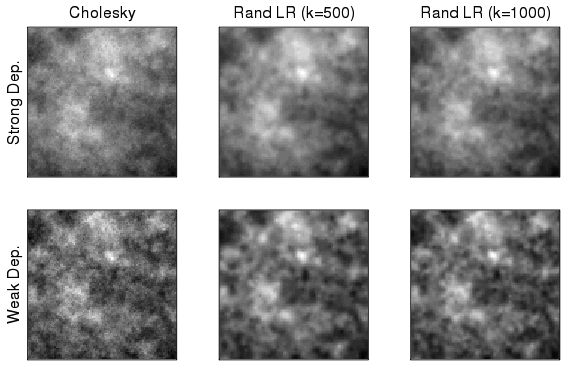
\includegraphics[width=\textwidth]{figs/RandLRPred.png}
\end{center}

\[ n=1000, \quad p=10000 \]

\end{frame}

\end{document}
